\chapter{TD4: Analyse Syntaxique (Antlr)}

\section{Ambition}

Comme dit dans l'introduction, le but de ce TD était de se familiariser avec l'environnement Antlr dans l'optique, à terme, d'avoir une grammaire prenant en entrée une phrase ``\textit{lemmatisée}'' pour en ressortir une requête SQL.

\medskip

Le TD en lui-même ne requérait pas de création de classes Java particulières. La génération de la grammaire se faisait à partir du logiciel AntlrWorks. Ce logiciel, après avoir ouvert un fichier \lstinline{.g} permet de générer les classes Java qui seront directement utilisées dans le projet Eclipse.

\section{Analyses préliminaires}

Après avoir compris comment une grammaire fonctionnait, il nous a fallu nous intéresser à la structuration d'une requête SQL afin d'un tirer des \textit{patterns} que l'on traduirait dans notre grammaire. Nous sommes pour cela partis du fichier de grammaire d'exemple fourni dans le cadre du TD.

\medskip

Au préalable, avant d'aboutir à une requête SQL, nous avons dû analyser les requêtes en langage naturel susceptibles d'être entrées par les utilisateurs. Par exemple :

\fakeshell
\begin{lstlisting}
Je veux les fichiers qui parlent de Zuckerberg.
Je veux les numéros qui ont été écrits en mai 2011.
Afficher les fichiers de la rubrique Focus.
Je voudrais les fichiers datant de 2012 et parlant de tempête.
\end{lstlisting}
\java

\subsection{Analyse de la requête en langage naturel}

Dans les exemples donnés ci-dessus, on constate plusieurs choses :

\begin{itemize}
    \item \textbf{La première partie} de la requête contient un verbe d'action (ex: ``Je veux'')
    \item \textbf{La seconde partie} contient les informations que l'on cherche à obtenir (ex: ``les numéros'', ``les fichiers')
\end{itemize}

\sql
Ces deux parties correspondront aux clauses \lstinline{SELECT} et \lstinline{FROM} de notre requête SQL. Les tables SQL dans lesquelles rechercher seront déterminées en fonction du type d'information que l'on souhaite ; toutes les tables ne contiennent pas les mêmes types d'informations (certaines contiennent des dates, des numéros d'articles, des rubriques, etc).

\medskip

Puis, le reste des phrases peut être défini comme ceci :

\begin{itemize}
    \item \textbf{La troisième et dernière partie} de la requête contient des contraintes de recherche, c'est-à-dire des conditions sur les informations (ex: ``qui parlent de Zuckerberg'', ``de la rubrique Focus''). Ces conditions peuvent être sous-catégorisées :
    \begin{itemize}
        \item Un mot particulier doit être présent
        \item Une rubrique
        \item Une date
    \end{itemize}
\end{itemize}

Cela signifie que ces conditions seront nos clauses \lstinline{WHERE} en SQL. Cette troisième partie de la requête contient de façon facultative un verbe de recherche (ex: ``qui parlent'').

\subsubsection{Verbe d'action}\label{action}

Il convenait donc de commencer à remplir notre fichier de lexique (contenant nos lemmes) avec les verbes d'action. Nous avons retenu le mot ``vouloir'' qui sera détecté plus tard par notre grammaire. Ainsi, nous avons fait correspondre plusieurs verbes (avec quelques formes conjuguées) au mot ``vouloir'' dans notre lexique, comme ceci :

\code{Extrait de nos lemmes}
\begin{lstlisting}
veux       vouloir
afficher   vouloir
lister     vouloir
\end{lstlisting}

\sql
\subsubsection{Informations (clause \lstinline{SELECT})}

Concernant les mots tels que ``numéros'' ou ``fichiers'', nous nous sommes assurés que le lexique de lemmes fournis dans le cadre du TP mettait bien ces mots au singulier. Dans le cas contraire nous avons dû ajouter la forme au singulier dans notre lexique de lemmes afin d'avoir une recherche fonctionnelle (car les noms des colonnes dans les tables SQL sont au singulier), comme cela a été le cas avec le mot ``fichiers'' auquel nous avons fait correspondre ``fichier''.

\subsubsection{Verbe de recherche}

Comme dit plus haut, nous avons dans un premier temps décidé que la recherche avec \sql\lstinline{WHERE} pourrait porter sur trois critères : une date, une rubrique ou des mots.

\medskip

Pour les mots, il s'agissait ici de faire la même chose que pour le verbe d'action (voir sous-section \ref{action}). Nous avons choisi d'utiliser le mot ``contenir'' comme verbe de recherche lorsque l'on souhaite une recherche SQL du type \lstinline{WHERE mot = 'x'}. Nous avons donc ajouté plusieurs synonymes à notre lexique, comme ceux-ci par exemple :

\code{Nos lemmes}
\begin{lstlisting}
contiennent  contenir
contenant    contenir
contient     contenir
concernant   contenir
comprenant   contenir
concernant   contenir
parlant      contenir
...
\end{lstlisting}

Concernant des recherches sur la rubrique ou la date, parfois il n'y a pas de verbe de recherche, comme dans la phrase ``Afficher les fichiers de la rubrique Focus''. Il faudra donc dans notre grammaire être capable de générer nos clauses \lstinline{WHERE}, en fonction de la présence éventuelle d'un verbe ou directement en fonction du paramètre. Ici, pour rubrique, cela sera assez facile dans le sens où le mot ``rubrique'' peut être repéré aisément.

\medskip

Dans les cas où cela n'est pas possible aussi facilement et en l'absence de verbe, il faudra utiliser une autre méthode. \textbf{Une solution envisageable que nous avons utilisée dans le projet est un pré-traitement de la requête lemmatisée, avant qu'elle soit transmise à l'analyseur grammatical}. Par exemple, pour une date, une requête en langage naturel pourrait finir par ``... écrits en 2011''. ``écrits en'' précède la date mais ces deux mots sont retirés lors de la lemmatisation car présents dans la stop list. Notre pré-traitement va donc essayer de détecter des jours, mois de l'année ou des années et ensuite rajouter devant le mot ``date'' qui sera lui utilisé par la grammaire.\\
Nous avons également veillé à remplacer les mois par leurs équivalents en chiffres dans notre pré-traitement.\\
En somme et par exemple, une requête lemmatisée telle que :

\code{Requête lemmatisée}
\begin{lstlisting}
vouloir article mai 2011
\end{lstlisting}
deviendra comme ceci, à la sortie de notre pré-traitement :
\code{Requête lemmatisée formatée}
\begin{lstlisting}
vouloir article date 05 2011
\end{lstlisting}

\bigskip

Enfin, concernant une recherche plus complexe incluant rubrique et/ou date et portant sur un ou plusieurs mots, il faudra que la liste des mots soit précédée de ``contenir'' et que les mots soient séparés par le conjonctif ``et'' ou ``ou''. Les mots ``et'' et ``ou'' sont respectivement remplacés par ``and'' et ``or'' grâce à notre dictionnaire de lemmes. On acceptera plusieurs suites de mots, qui généreront quelque chose comme ceci :

\code{Requête lemmatisée formatée}
\begin{lstlisting}
vouloir fichier contenir avion and chasse and rubrique focus and date 2011 and contenir militaire
\end{lstlisting}

Cela implique que le mot ``contenir'' soit un lemme ayant remplacé un mot de même sens tapé par l'utilisateur, et qu'il soit placé à chaque fois avant le groupe de mots. Il est donc primordial que la requête en langage naturel soit bien structurée, telle que :

\code{Exemple de requête en langage naturel}
\begin{lstlisting}
Je veux les fichiers parlant d'avion et de chasse, dans la rubrique focus, datés de 2011, et contenant le mot militaire.
\end{lstlisting}

\subsubsection{Conséquences}

Tout cela implique donc que l'on devra se passer de mots ``contenir'', ``et'', ``ou'', ``rubrique'' et ``date'' comme critères de recherche. Nous ne pourrons pas chercher d'élément dans la base de données contenant un de ces mots. Une requête en langage naturel interdite serait pas exemple :

\code{Requête impossible à faire}
\begin{lstlisting}
Je veux les fichiers parlant de rubrique
\end{lstlisting}

De manière générale, tous les mots que nous avons ajoutés à notre stop list ne pourront pas servir pour faire une recherche sur un mot.

\subsection{Analyse de la structure d'une requête SQL}

Il nous fallait maintenant écrire une grammaire qui permette d'analyser nos phrases lemmatisées et pré-formatés afin d'obtenir des requêtes SQL viables. Une requête SQL est généralement de la forme :

\sql
\begin{lstlisting}
SELECT a,b,c FROM X,Y WHERE x = y AND w = z;
\end{lstlisting}
Dans cet exemple il y a deux conditions \lstinline{WHERE} mais on peut très bien en imaginer une seule ou plusieurs.

\medskip

On constate donc que la forme d'une requête SQL est semblable à notre requête en langage naturel lemmatisée et préformatée. Tout d'abord le verbe d'action (\lstinline{SELECT}), les informations à rechercher et où les chercher (\lstinline{a,b,c FROM X,Y}), et enfin les conditions de recherche (\lstinline{WHERE x = y AND w = z}).

\medskip

Il est donc aisé de repérer les clauses \lstinline{SELECT} et \lstinline{WHERE}. En revanche, en ce qui concerne les conditions \lstinline{WHERE}, cela est plus compliqué, et ce pour plusieurs raisons :

\begin{itemize}
  \item La condition peut porter sur 0, 1 ou plusieurs \textbf{mots}
  \item La condition peut porter sur la rubrique
  \item La condition peut porter sur la date
\end{itemize}

Toutes ces conditions peuvent être dans n'importe quel ordre. C'est principalement ici que réside la difficulté. Il faut de plus être capable de détecter tous les critères de recherche, qui sont potentiellement aussi nombreux qu'il y a de colonnes différentes dans les tables SQL.

\medskip

Jusqu'à aujourd'hui (date de rédaction de ce présent rapport), nous avons décidé de nous concentrer sur trois critères :

\begin{itemize}
    \item Recherche sur un mot ou plusieurs mots
    \item Recherche sur une rubrique
    \item Recherche sur une date (mois et/ou année)
\end{itemize}
On pourra bien sûr faire une recherche sur un mot et une rubrique, deux mots et une rubrique et une date, etc.

\medskip

Nous avons également essayé de prendre en considération plusieurs critères séparés par les conjonctures \lstinline{ET} ou \lstinline{OU}.
Pour la recherche sur un mot, nous faisons le choix d'effectuer celle-ci à la fois sur le texte uniquement (dans un premier temps), c'est-à-dire sur la colonne 'mot' de la table \lstinline{titretext}.

\medskip

Par la suite, d'ici à la fin du projet, nous essaierons de prendre en considération d'autres critères de recherche.

\subsection{Limites}

La principale contrainte de ce mode opératoire pour passer d'une requête en langage naturel à une requête SQL se pose au niveau de la transformation du langage naturel et le remplacement des termes (correction et pré-formatage). En effet afin de ``normaliser'' notre phrase tapée en entrée nous remplaçons certains voire tous les mots de la phrase par nos lemmes (issus de nos deux lexiques), ceci afin de pouvoir traduire cette phrase ``tokenizée'' en requête SQL. Cependant si nous faisons l'hypothèse d'une requête telle que ``\textit{Je veux les articles qui contiennent 'afficher' et 'concernant'}'', les mots ``afficher'' et ``concernant'' seront respectivement remplacés par ``vouloir'' et ``contenir'', ceux-ci étant des verbes d'action et de recherche et faisant donc partie des lemmes ; la requête initiale s'en verra donc modifiée. \textbf{Cela avait été dit plus haut dans ce rapport mais il est important de le rappeler.}

\section{Création de la grammaire}

Voici un schéma qui explique comment est analysée une phrase en entrée par notre grammaire :

\begin{figure}[H]
    \centering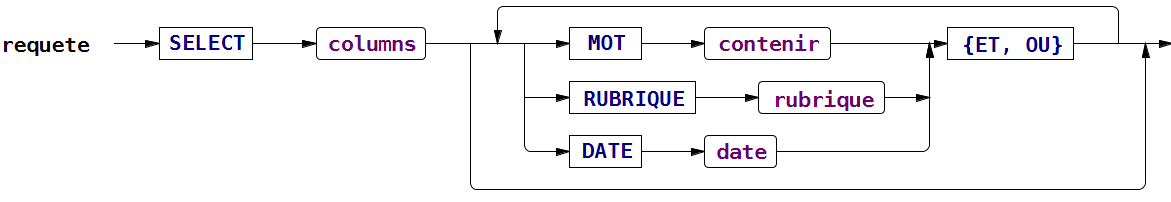
\includegraphics[width=1\textwidth]{images/grammaire.png}
    \caption{Génération d'arbre associé}
\end{figure}

\begin{figure}[H]
    \centering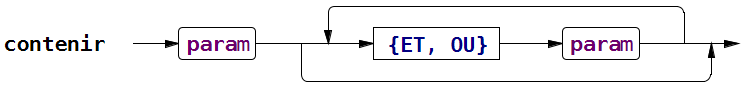
\includegraphics[width=1\textwidth]{images/param.png}
    \caption{Gestion de plusieurs paramètres avec conjectures}
\end{figure}

\begin{figure}[H]
    \centering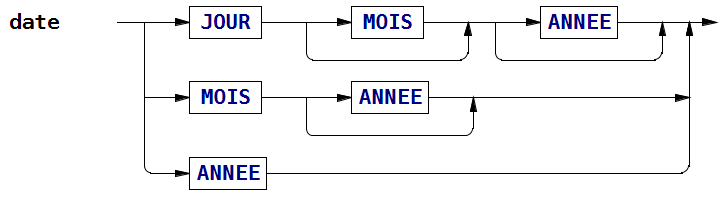
\includegraphics[width=1\textwidth]{images/date.png}
    \caption{Gestion des dates}
\end{figure}

\subsection{Règles}

Voici les règles que nous avons définies pour arriver à ce résultat :

\code{Règles}
\begin{lstlisting}
SELECT:'vouloir';

COLUMNS: 'fichier'|'numero'|'mot'|'email';

ET:'and';
OU:'or';

MOT:'contenir';

RUBRIQUE:'rubrique';

DATE:'date';
MOIS:('0'('1'..'9'))|'10'|'11'|'12';
ANNEE:('1'|'2')'0'..'9''0'..'9''0'..'9';
JOUR:('0'..'9')|(('1'|'2')'0'..'9')|'30'|'31';

WS:(' ' |'\t' | '\r' | 'je' | 'qui' | 'dont') {skip();} | '\n';

VAR:('A'..'Z' | 'a'..'z'|'\u00a0'..'\u00ff')(('a'..'z')|('0'..'9')|'-'|('\u00a0'..'\u00ff'))+;
\end{lstlisting}

À noter que l'ordre des tokens tel qu'il est donné dans la grammaire influe sur le parcours de l'arbre dans celle-ci et donc sur le traitement de la requête. Nous avons veillé à bien ordonner nos tokens.

\medskip

Ces règles sont assez explicites pour ne pas avoir besoin d'être expliquées, les explications fournies dans les sections précédentes étant suffisantes. On peut cependant préciser que \lstinline{WS} permet de ne pas tenir compte de certaines chaînes de caractères.

\section{Résultat actuel}

Exemple avec la phrase lemmatisée: \textit{vouloir fichier contenir voiture and rubrique focus and date 05 2011 and}.

\begin{figure}[H]
    \centering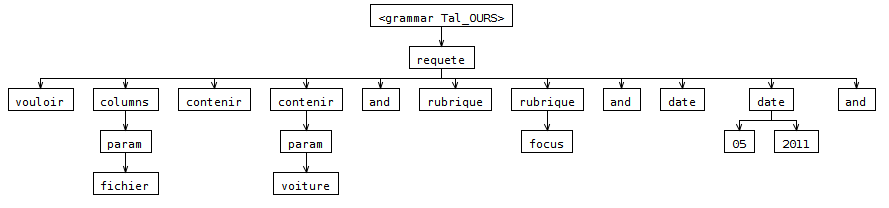
\includegraphics[width=1\textwidth]{images/arbre.png}
    \caption{Arbre généré}
\end{figure}

\noindent Ici, le ``and'' final sera retiré dans le post-traitement (qui est une méthode que l'on execute après avoir récupéré la requête SQL).

\bigskip
\bigskip

À l'heure actuelle, notre grammaire accepte des requêtes assez simples mais précises. Il conviendra d'ici à la fin du projet de considérer peut-être des recherches sur l'email, uniquement les titres, etc. Il faudra probablement étoffer notre post-traitement, qui est appliqué à la requête générée par Antlr, pour supporter également les \sql\lstinline{INNER JOIN}, nécessaires lors des recherches sur un texte contenant plusieurs mots.
